%%%%%%%%%%%%%%%%%%%%%%%%%%%%%%%%%%%%%%%%%%%%%%%%%%%%%%%%%%%%%%%%%%%%%%


%%% Preamble
\documentclass[paper=a4, fontsize=11pt]{scrartcl}
\usepackage[T1]{fontenc}
\usepackage{fourier}

\usepackage[english]{babel}															% English language/hyphenation
\usepackage[protrusion=true,expansion=true]{microtype}	
\usepackage{amsmath,amsfonts,amsthm} % Math packages
\usepackage[pdftex]{graphicx}	
\usepackage{url}

%% BEGIN ADDED FOR FAQ Section
\usepackage[margin=1in]{geometry} % Required to make the margins smaller to fit more content on each page
\usepackage[linkcolor=blue]{hyperref} % Required to create hyperlinks to questions from elsewhere in the document
\hypersetup{pdfborder={0 0 0}, colorlinks=true, urlcolor=blue} % Specify a color for hyperlinks
\usepackage{todonotes} % Required for the boxes that questions appear in
\usepackage{tocloft} % Required to give customize the table of contents to display questions
\usepackage{microtype} % Slightly tweak font spacing for aesthetics

% Create the command used for questions
\newcommand{\question}[1] % This is what you will use to create a new question
{
\refstepcounter{questions} % Increases the questions counter, this can be referenced anywhere with \thequestions
\par\noindent % Creates a new unindented paragraph
\phantomsection % Needed for hyperref compatibility with the \addcontensline command
\addcontentsline{faq}{questions}{#1} % Adds the question to the list of questions
\todo[inline, color=gray!10]{\textbf{#1}} % Uses the todonotes package to create a fancy box to put the question
\vspace{1em} % White space after the question before the start of the answer
}
%% END QUESTION ADD

% Algorithms package
\usepackage{fancybox}
\usepackage{algorithm}
\usepackage{caption}
\usepackage{algorithmic}
\usepackage{bbm}


%%% Custom sectioning
\usepackage{sectsty}
\allsectionsfont{\centering \normalfont\scshape}


%%% Custom headers/footers (fancyhdr package)
\usepackage{fancyhdr}
\pagestyle{fancyplain}
\fancyhead{}											% No page header
\fancyfoot[L]{}											% Empty 
\fancyfoot[C]{}											% Empty
\fancyfoot[R]{\thepage}									% Pagenumbering
\renewcommand{\headrulewidth}{0pt}			% Remove header underlines
\renewcommand{\footrulewidth}{0pt}				% Remove footer underlines
\setlength{\headheight}{13.6pt}


%%% Equation and float numbering
\numberwithin{equation}{section}		% Equationnumbering: section.eq#
\numberwithin{figure}{section}			% Figurenumbering: section.fig#
\numberwithin{table}{section}				% Tablenumbering: section.tab#


%%% Maketitle metadata
\newcommand{\horrule}[1]{\rule{\linewidth}{#1}} 	% Horizontal rule

\title{
		%\vspace{-1in} 	
		\usefont{OT1}{bch}{b}{n}
		\normalfont \normalsize \textsc{PacBio Variant Calling Group} \\ [25pt]
		\horrule{0.5pt} \\[0.4cm]
		\huge The Old (Heuristic) versus New (Probablistic) Scoring Models\\
		\horrule{2pt} \\[0.5cm]
}
\author{
		\normalfont 								\normalsize
        Nigel Delaney\\[-3pt]		\normalsize
        \today
}
\date{}


%%% Begin document
\begin{document}
\maketitle

\section{Introduction}

This document shows some simple tweaks to the old model for $P(R|T)$ that convert it into a probabilistic framework so that we can optimize it using maximum likelihood.  It assumes there are no QV values associated with the reads, and so represents a `constant rate' model.   This model has 29 parameters and can easily be fitted with maximum likelihood.  It is designed to represent a baseline model against which the utility of QV values can be assessed.  

The recursions required for the likelihood calculation in this model are nearly identical to the current recursions, so require almost no code changes.  It also makes the central assumption that all the transition probabilities are shared across latent states, as shown in Figure 1, so only requires one $I \times J$ matrix to perform the recursion, .


\begin{figure}[H] %% The [h] means place the figure here.
	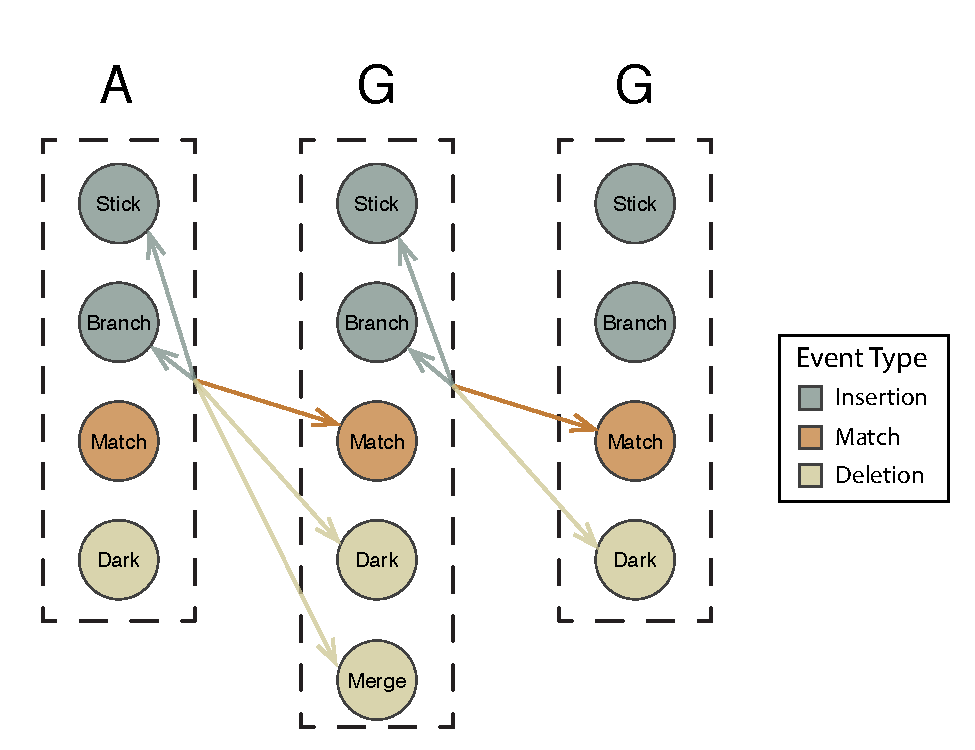
\includegraphics{CCSScoring}
		\caption{The generative model for reads given a template.  The transition probabilities out of each latent state enclosed in the same dashed box are all equal, greatly reducing the parameters needed and the computational complexity of the likelihood algorithm.  Transitions are determined by the next basepair present in the template, with a merge move possible if it matches the current template.  All possible transitions are indicated by arrows.}
\end{figure}


\section{Model Parameters and Estimation}
 
 The transitions between states are governed by two adjacent nucleotides, which determines how frequently different moves occur.  Therefore, for a complete model we want to model the transition probabilities as a function of the two neighboring basepairs, with one set of parameters if they occur as a dinucleotide (which allows for a merge move) and another set if they do not (so that a merge is not possible).  Note that at template position $j$, the transitions are governed by the \textit{next} template position, not the current one.  I will consider 8 possible template contexts, one for each homopolymer and non-homopolymer context possible:
  
 
 \begin{center}
 \texttt{GG \\
NG \\
AA \\
NA \\
CC \\
NC 
 }
 \end{center}
 
 Depending on if the context is or is not a homopolymer, there are either 5 or 4 transition parameters needed.
 
 \begin{center}
$\theta_{\text{Homopolymer}} = [p_{Match}, p_{Stick}, p_{Branch}, p_{Deletion}, p_{Merge} ]$
 \\
$ \theta_{\text{Regular}} = [p_{Match}, p_{Stick}, p_{Branch}, p_{Deletion}]$
\end{center}

Additionally, we need to estimate the global miscall probability $\epsilon$, since all transition parameters must sum to one, this means there are a total of $ (4 -1) \times 4 + (5-1) \times 4 + 1 = 29$ free parameters to estimate.  Although we could condense the model so that the relative transition probabilities excluding the merge move were equal (thus requiring only 17 parameters), 29 parameters should be simple to fit and so this additional complexity will be allowed.  

  
\section{Old versus New Recursions}

In this section, I just give the steps for calculating the different recursions for both the new framework and the old for comparison.  Note that the probabilities shown depend on the di-nucleotide context, which governs the relative parameters given.  Also, since this is a CRF/HMM model, each probability is the simple product of the probability of being in the previous state, transitioning to the new state, and emitting the value there.

\subsection{\textbf{Match Score}}


\textbf{Simple Scoring Version}

\[
	\text{Match Score} = \alpha_{i-1,j-1}  +  \begin{cases}
							 \ \text{A fixed value} & \text{if }  R_{i} = T_{j} \\
							 \text{Substitution score given for } R_{i} & \text{if }  R_{i}  \neq T_{j} 
							 \end{cases}
\]

\textbf{Probabilitistic Scoring Version}

\[
	\text{Match Score} = \alpha_{i-1,j-1}  \times p_{\rightarrow Match} \times  \begin{cases}
							 (1 - \epsilon) & \text{if }  R_{i} = T_{j} \\
							 \frac{1}{3} \cdot \epsilon & \text{if }  R_{i}  \neq T_{j} 
							 \end{cases}
\]

Note that in the simple scoring version, it just convolutes the two parameters and doesn't place any constraints on them.  The equation in the probability framework is the simple formula for the probability of that particular transition followed by that particular emission.  Also, the $\frac{1}{3}$ value simply represents a uniform prior over incorrectly admitted bases, though it might be better to consider each emission probability separately.


 
\subsection{\textbf{Insertion Score}}


\textbf{Simple Scoring Version}
\[
	\text{Insertion Score} = \alpha_{i-1,j}  +  \begin{cases}
							 \text{Insertion score  for } R_{i} \text{ scaled to a branch step} & \text{if }  R_{i} = T_{j+1} \\
							 \text{Insertion score  for } R_{i} \text{ scaled to a non-branch step} & \text{if }  R_{i}  \neq T_{j+1} 
							 \end{cases}
\]

\textbf{Probabilitistic Scoring Version}

\[
	\text{Insertion Score} = \alpha_{i-1,j}  \times  \begin{cases}
							 p_{\rightarrow \text{Branch}} \cdot 1   & \text{if }  R_{i} = T_{j+1} \\
							 p_{\rightarrow \text{No-Branch}}  \cdot \frac{1}{3} & \text{if }  R_{i}  \neq T_{j+1} 
							 \end{cases}
\]

Note that in the simple scoring version we assume that we know from the data exactly if the observation was due to a branch or non-branch.  In the probability version, we express this as a condition that a branch cannot emit the next basepair of the read if it is a non-branch step.  In actuality, we should probably allow such emissions and change the model.


\subsection{\textbf{Deletion Score}}

\textbf{Simple Scoring Version}

\[
	\text{Deletion Score} = \alpha_{i,j-1}  +  \begin{cases}
							 \text{Deletion score  for } R_{i+1}  & \text{if }  \text{DeletionTag}_{i+1} = T_{j} \\
							 \text{A fixed constant} & \text{if }  \text{DeletionTag}_{i+1} \neq T_{j} 
							 \end{cases}
\]

\textbf{Probabilistic Scoring Version}

\[
	\text{Deletion Score} = \alpha_{i,j-1}  \times  \begin{cases}
							 p_{ \rightarrow \text{Deletion}} \cdot 1 & \text{if }   T_{j} \neq T_{j+1} \\
							 p_{ \rightarrow \text{Deletion}} \cdot 1 + p_{\rightarrow \text{Merge}}  \cdot 1  & \text{if }  T_{j} = T_{j+1} 
	\end{cases}
\]

I think the DeletionTag is adds more problems than it solves, so dropped it.  Also, the merge move is now explicitly incorporated as a deletion step, and multiple merges are allowed.
 
 
\section{Model Fitting}

Since this is a constant model, we can use Baum-Welch to easily estimate the parameters.  This is just dynamic programming followed by counting.  However, unlike calculating the likelihood where we only need one $I \times J$ matrix, in order to use Baum-Welch we will need 2 separate $I \times J$ matrices for each state to calculate the forwards and backward probabilities.

\subsection{$\epsilon$ Estimation}

To estimate the mis-emission probability, we simply look at the $I \times J$ Matrix which represents a match.  We sum up over each element in this matrix, weighting by the total probability based on the forward and backward matrix. 
\begin{center}
$\hat{ \epsilon} = \frac{\sum\limits_{i=1}^I \sum\limits_{j=1}^J F(i,j) \cdot B(i,j) \cdot \mathbbm{1}_{R_{i} = T_{j}} }  {\sum\limits_{i=1}^I \sum\limits_{j=1}^J F(i,j) \cdot B(i,j)}$
\end{center}

\subsection{Transition Parameter Estimation}

Since we are training transition parameters for 8 different contexts, we first need to group all template columns according to which of the 8 different di-nucleotide contexts they belong to.  Once we have done that, we simply iterate the same method for each group.

We simply need to calculate the recursively calculate for each element, the expected number of times a transition occured.

For example, although we need to calculate them separately, for insertion transitions, we calculate the probability of being in the previous state (if at position $i,j$, sum of all matrices $F(i-1, j)$ positions).  We then calculate the probability of transition using the current parameters as 

\begin{center}
$(\sum F(i-1, j) )\times p_{\rightarrow insertion} \times p_{emission}  \times B(i, j) $
\end{center}

Where the probability of emission is either $0$, $\frac{1}{3}$ or $1$ depending on the type of insertion and context being considered.


Analogous results are used for Match and Deletion columns, with the only change being that they sum over the upper diagonal and left hand matrix positions. 

 
%%% End document
\end{document}